\section{Lab 1}
\subsection{Motivation}\label{sec:lab1_mot}
The motivation behind the first lab task was to create a PD regulator to the linearized
model of the helicopter \ref{eq:lin_model} for a cause to control its pitch. The equations
of motion can be find in \ref{eq:model_1}. For a simple visualization of the helicopter, see \ref{fig:helicopter_dia}.

\begin{subequations}\label{eq:model_1}
	\begin{align}
		\ddot{p}  &= -\frac{K_{f}l_{p}V_{d}}{J_{p}} = \frac{L_1Vd}{J_p} \label{eq:model_1_p} \\
		\ddot{e}  &= (2m_pgl_h-m_cgl_c)cos(e)+K_fl_hV_scos(p) = L_2cos(e)+L_3V_scos(p)\label{eq:model_1_e} \\
		\ddot{\lambda} &= \frac{l_hk_fV_scos(e)sin(p)}{J_{\lambda}} = L_4V_scos(e)sin(p) \label{eq:model_1_l} \\
	\end{align}
\end{subequations}

\subsection{Lab preperation}\label{sec:lab1_prep}
There were several tasks which needed to be done as preperation to the first lab day.
The first task was to derive the equations of motion from a given diagram of the helicopter \ref{fig:helicopter_dia}.
This task required thoroughly analyzing the forces which the helicopter is affected by.
When this was done, it was needed to linearize the model around the equlibrium (all system states equal zero) represented by \ref{fig:helicopter_dia} such that 
creating controllers would be easier. We were now ready to implement a PD controller given by \ref{eq:PD}
and insert this into the linearized equation of pitch acceleration, to control the pitch to a given reference.
The last preperation for lab 1 was to make a test plan for pole placements to the pitch control. We used the equations in \ref{eq:pole_place}.

\begin{subequations}\label{eq:lin_model}
	\begin{align}
        \tilde{V_d} &= V_d-V_{d,origo} = V_d\\
        \tilde{V_s} &= V_s-V_{s,origo} = V_s+\frac{L_2}{L_3}\\
		\ddot{p}  &= \frac{L_1\tilde{V_d}}{J_p} = K_1V_d\label{eq:lin_p} \\
		\ddot{e}  &= \frac{L_3\tilde{V_s}}{J_e} = K_2\tilde{V_s}\label{eq:lin_e} \\
		\ddot{\lambda} &= \frac{L_4L_2\tilde{p}}{L_3J_{\lambda}} = K_3p\label{eq:lin_l} \\
	\end{align}
\end{subequations}
\begin{subequations}\label{eq:PD}
	\begin{align}
        V_d &= K_{pp}(pc-p)-K_{pd}\dot{p}
	\end{align}
\end{subequations}
\begin{subequations}\label{eq:pole_place}
	\begin{align}
    K_{pd} &= -\frac{s_2+s_1}{K_1}\\
    K_{pp} &= \frac{s_2(s_2-s_1)}{K_1(\frac{s_2}{s_1}-1)}
	\end{align}
\end{subequations}

\subsection{Hypotheses/Test plan}
We wanted to expirement the controller by setting the poles at several different positions, including real and complex numbers.
We prepared twelve different tests, with hyoptheses coming from control theory which as for poles in LHS of s plane are exponentially stable, RHS are unstable and poles in origo are stable.
The table \ref{tab:testskjema_lab1} gives an overview of our tests and their s-values, stability result and hypotheses.
During the tests we have a step equal 10V in the disturbance of the system from 15s to 15.2s. We also added a step in the elevation reference equal -0.55 until 5 seconds have past.
\begin{table}[h]
\centering
\phantomsection % Creates an anchor for the hyperlink
 % Place the label at the top of the table
    \begin{tabular}{||c c c c c||} 
     \hline
     Test & Poles & Pitch ref & Hypotheses & Result \\ [0.5ex] 
     \hline\hline
     1 & -1,-1 & 0 & Exp. Stability & Exp. Stability \\ 
     \hline
     2 & -5,-5 & 0 & Exp. Stability & Exp. Stability \\
     \hline
     3 & $-1\pm j5$  & 0 & Exp. Stability & Exp. Stability  \\
     \hline
     4 & $-1\pm j$ & 0 & Exp. Stability & Exp. Stability \\
     \hline
     5 & $-5\pm j$ & 0 & Exp. Stability & Exp. Stability \\  
     \hline
     6 & $-5\pm j5$ & 0 & Exp. Stability & Exp. Stability \\ 
     \hline
     7 & $\pm j$ & 0 & Marginal Stability & Unstable \\  
     \hline
     8 & $\pm j5$ & 0 & Marginal Stability & Unstable \\ 
     \hline
     9 & $0$ & 0 & Marginal Stability & Unstable \\ 
     \hline
     10 & $1\pm j$ & 0 & Unstable & Unstable \\ 
     \hline
     11 & -1,1 & 0 & Unstable & Unstable \\ 
     \hline
     12 & 1,1 & 0 & Unstable & Unstable \\ [1ex]
     \hline
    \end{tabular}
    \caption{Test scheme}
    \label{tab:testskjema_lab1}
\end{table}
\subsection{Results}
We have decided to plot results of only five of the done tests, such that the plots are not redundant.
The plot \ref{fig:pitch_plot} visualize a time series for test 1,4,7,9 and 11. Y-axis is the pitch measured in radians. X-axis shows each timestep. The reason behind this is to include different pole-values which
with also different specific hypotheses and result. For all tests the reference of the pitch was at 0 rad. The step functions in elevation reference and disturbance are specifically visible for test 1 and test 4. 
At around 5 seconds the pitch seems to be affected by the elevation going to 0, and the pitch has even bigger response to the step in disturbance at 15 seconds. The controller manages to send the pitch back around zero 
fairly fast and smooth. 

When looking at plot \ref{fig:pitch_plot} test 9 and test 11 is cut off early. The reason behind this is that 
the pitch became so unstable, where at a point it could provide harm to the helicopter. As safety measure we cut its power early. 
Test 1 and 4 have a similar run, which is expected as they both have same real part. However even though test 4 have an imaginary part, 
it dosent seem to add more swings than the one without an imaginary part.

\begin{figure}[h!]
    \centering
    \subfloat[Plots from test 1 and 4]{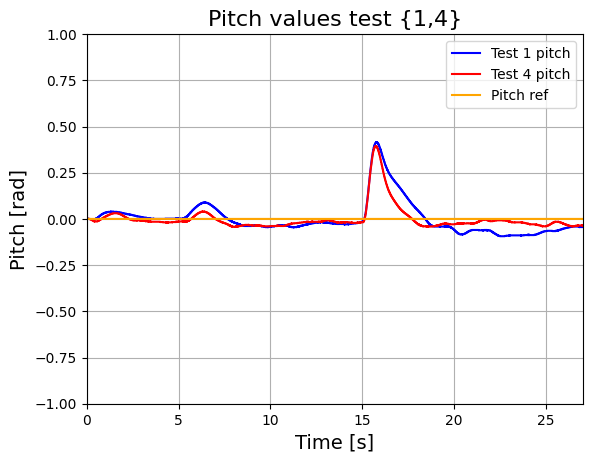
\includegraphics[width=0.5\textwidth]{figures/lab1pitchV1.png}}\hfill
    \subfloat[Plots from test 7,9 and 11]{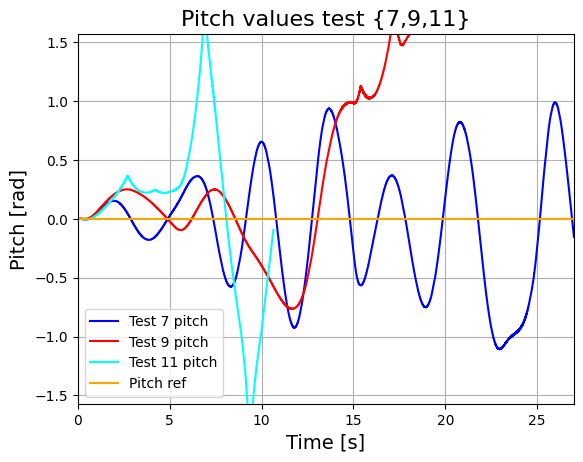
\includegraphics[width=0.5\textwidth]{figures/lab1pitchV2.png}}
    \caption{Timeseries of pitch angle in [rad].}
    \label{fig:pitch_plot}
\end{figure}     

\subsection{Conclusion}
The results match our hypotheses for the tests well. Poles in left hand side of the s plane give exp. stability and poles in right hand side give unstability. However if the real parts of the poles were close to the 
imaginary axis, the closed loop system became unstable. This is likely a result of the real system being heavily unlinear, 
and us working with a simple linearized model of it, leaving several margins of error. Sadly when saving data from the lab day we didnt accompany time series of the controller output, which would be a valuable asset to discuss in this report. 
It would be interesting to visualize and compare values the PD controller generated throughout the tests.  

